\documentclass[a4paper,11pt]{article}
\usepackage{nopageno} % visto che in questo caso abbiamo una pagina sola
\usepackage{lmodern}
\renewcommand*\familydefault{\sfdefault}
\usepackage{sfmath}
\usepackage[utf8]{inputenc}
\usepackage[T1]{fontenc}
\usepackage[italian]{babel}
\usepackage{indentfirst}
\usepackage{graphicx}
\usepackage{animate}
\usepackage{tikz}
\usepackage{wrapfig}
\newcommand*\circled[1]{\tikz[baseline=(char.base)]{
		\node[shape=circle,draw,inner sep=2pt] (char) {#1};}}
\usepackage{enumitem}
% \usepackage[group-separator={\,}]{siunitx}
\usepackage[left=2cm, right=2cm, bottom=2cm]{geometry}
\frenchspacing

\newcommand{\num}[1]{#1}

% Macro varie...
\newcommand{\file}[1]{\texttt{#1}}
\renewcommand{\arraystretch}{1.3}
\newcommand{\esempio}[2]{
\noindent\begin{minipage}{\textwidth}
\begin{tabular}{|p{5cm}|p{11cm}|}
	\hline
	\textbf{da \file{stdin}} & \textbf{su \file{stdout}}\\
	\hline
	\tt \small #1 &
	\tt \small #2 \\
	\hline
\end{tabular}
\end{minipage}
}

\newcommand{\sezionetesto}[1]{
    \section*{#1}
}

\newcommand{\gara}{Esame algoritmi 2021-07-21 VR}

%%%%% I seguenti campi verranno sovrascritti dall'\include{nomebreve} %%%%%
\newcommand{\nomebreve}{}
\newcommand{\titolo}{}

% Modificare a proprio piacimento:
\newcommand{\introduzione}{
%    \noindent{\Large \gara{}}
%    \vspace{0.5cm}
    \noindent{\Huge \textbf \titolo{}~(\texttt{\nomebreve{}})}
    \vspace{0.2cm}\\
}

\begin{document}

\renewcommand{\nomebreve}{hanoi\_split}
\renewcommand{\titolo}{Split even and odd disks of an Hanoi tower\\}

\introduzione{}

Studiamo una variante del puzzle della torre di Hanoi. Se non conosci la versione classica o la descrizione quì sotto non basta, sei libero di cercare in internet o sperimentare col seguente applet:

\begin{verbatim}
https://www.mathsisfun.com/games/towerofhanoi.html
\end{verbatim}

Ci sono tre pioli ($A$,$B$ e $C$) su cui sono collocati $n$ dischi numerati da $1$ ad $n$ (dal più piccolo al più grande). Le \emph{configurazioni valide} sono quelle in cui nessun disco si trova collocato sopra un disco più piccolo.
La \emph{configurazione iniziale} è l'unica valida in cui tutti i dischi sono collocati sul piolo $A$.

\begin{figure}[h!]
\begin{center}
  \noindent 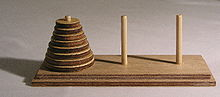
\includegraphics[width=0.57\textwidth]{figures/220px-Tower_of_Hanoi.jpeg}
\end{center}
\caption{Configurazione iniziale $A^8$ del puzzle per $n=8$.}
\end{figure}

Qualsiasi sia il numero di dischi $n$, il tuo obiettivo è quello di portarti dalla configurazione iniziale alla \emph{configurazione finale standard} spostando sempre un solo disco alla volta (mossa) e visitando solo configurazioni valide.
Nel puzzle classico offerto da Édouard Lucas (1883) la configurazione finale è quella con tutti i dischi collocati sul piolo $C$, ed è celebre l'elegante soluzione ricorsiva che lo risolve nel minimo numero di mosse. La soluzione ottima è di fatto unica anche se trova diverse descrizioni/rappresentazioni/interpretazioni.

Noi proponiamo di considerare come configurazione finale quella in cui ciascun disco~$i$ con~$i$ dispari è sul piolo $B$ mentre tutti gli altri dischi sono sul piolo $C$. Ti anticipiamo che anche nella nostra variante la soluzione ottima sarà unica.\\

In realtà vogliamo valutare e consentire l'espressione di diverse competenze. Nei subtask di tipo~$t=1$ ti chiediamo di listare tutte le mosse di una soluzione ottima, che impieghi il minor numero possibile di mosse.
Nei subtask di tipo~$t=0$ ti chiediamo solamente di computare tale numero di mosse, senza doverle generare, ma più velocemente.
Nel primo caso l'approccio ricorsivo è fortemente consigliato anche nella stesura del codice, e probabilmente ti converrà affrontare prima questi subtask di tipo~$t=1$.


\sezionetesto{Input ed Output}

Per la gestione pulita di input ed output consigliamo di utilizzare il template di soluzione fornito tra gli attachments alla pagina del problema.
Input ed output avvengono da \verb'stdin' e su \verb'stdout' rispettivamente.
La prima ed unica riga dell'input contiene i due numeri $t$ ed $n$, nell'ordine e separati da spazio. Questi indicano il tipo di richiesta: solo contare ($t=0$) o proprio listare una per una le mosse ($t=1$).

\indent
Nel caso in cui $t=0$ il vostro programma deve restituire su \verb'stdout' un unico numero naturale: il minimo numero di mosse che è necessario spendere per portare il gioco nella configurazione finale.

\indent
Nel caso in cui $t= 1$ il vostro programma deve riportare su \verb'stdout' tale sequenza di mosse che consente di raggiungere la configurazione finale. Il formato corretto è illustrato negli esempi.


% Esempi
\sezionetesto{Esempio di input/output}

In attachment alla pagina del problema trovate diverse coppie input/output tra cui le seguenti.


\vspace{0.5cm}
\esempio{1 3}{sposta il disco 1 dal piolo A al piolo B

sposta il disco 2 dal piolo A al piolo C

sposta il disco 1 dal piolo B al piolo C

sposta il disco 3 dal piolo A al piolo B

sposta il disco 1 dal piolo C al piolo B
}

\vspace{0.5cm}
\esempio{0 3}{5}

\vspace{0.5cm}
\esempio{0 4}{11}



\section*{Subtask}

  \begin{itemize}
    \item \textbf{Subtask 1 [0 punti]:} i casi di esempio forniti alla pagina del problema, essi includono i due casi sopra.
    \item \textbf{Subtask 2 [16 punti]:} $t=1$, $n \le 8$.
    \item \textbf{Subtask 3 [16 punti]:} $t=1$, $n \le 15$.
    \item \textbf{Subtask 4 [18 punti]:} $t=1$, $n \le 20$.
    \item \textbf{Subtask 5 [16 punti]:} $t=0$, $n \le 10$.
    \item \textbf{Subtask 6 [16 punti]:} $t=0$, $n \le 20$.
    \item \textbf{Subtask 7 [18 punti]:} $t=0$, $n \le 40$.
  \end{itemize}
  


\end{document}
